% Created 2022-11-05 六 00:14
% Intended LaTeX compiler: xelatex
\documentclass[]{beamer}
\usepackage{graphicx}
\usepackage{longtable}
\usepackage{wrapfig}
\usepackage{rotating}
\usepackage[normalem]{ulem}
\usepackage{amsmath}
\usepackage{amssymb}
\usepackage{capt-of}
\usepackage{hyperref}
\usetheme{default}
\author{Jun Gao}
\date{\textit{<2022-11-04 五>}}
\title{INTENT INDUCE WITH SCCL AND OUT-DOMAIN DATA AUGMENTATION}
\hypersetup{
 pdfauthor={Jun Gao},
 pdftitle={INTENT INDUCE WITH SCCL AND OUT-DOMAIN DATA AUGMENTATION},
 pdfkeywords={},
 pdfsubject={},
 pdfcreator={Emacs 28.2 (Org mode 9.5.5)}, 
 pdflang={English}}
\begin{document}

\maketitle
\begin{frame}{Outline}
\tableofcontents
\end{frame}


\section{Introduction}
\label{sec:org231ae39}
\begin{frame}[label={sec:org922540b}]{dstc11}
\url{https://drive.google.com/file/d/1itlby2Ypq3sRVtOY1alr3ygjPZZdB2TT/view}
\end{frame}
\begin{frame}[label={sec:org4641558}]{sccl}
SCCL(supporting clustering with contrastive learning) is a deep clustering algorithm which can learning more adequate representation of short context. By using Contrastive Learning, same samples will be pull together while different ones will be pushing apart.

\begin{center}
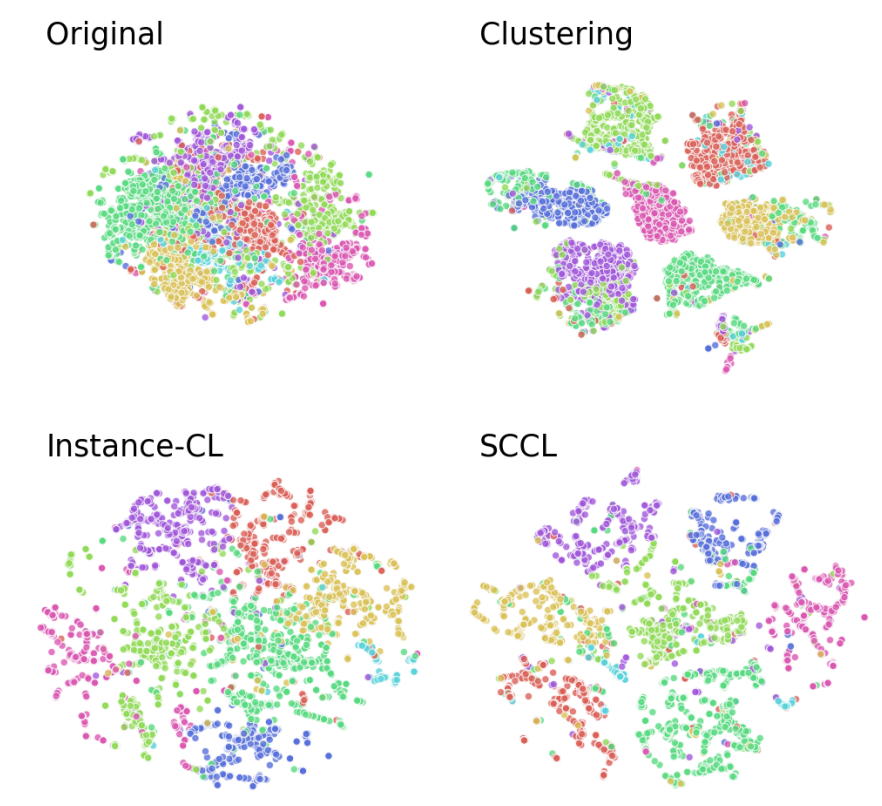
\includegraphics[width=0.5\textwidth]{../images/20221104-230515_screenshot.png}
\end{center}
\end{frame}
\section{our work}
\label{sec:org26907ee}
\begin{frame}[label={sec:orge47a25d}]{filtering high quality utterances with statistic rule or hdbscan}
In open intent induction, we will not have acess to the ground-truth utterances with intents, so need to filter out noise utterances. A tradition way is to use clustering algorithms, like hdbscan, but in this task, we find a more effective way to select high quality utterances, that is statistic rules. Specificlly, we count the highest frequency bi-gram phrase before the utterances in development dataset and find it domain-agnostic, thus we migrate the rule to test dataset and obtain high quality utterances.

For example, if "insurance\textsubscript{005}\textsubscript{001}" is a high quality utterance, "name is" is a bi-gram phrase before it.

\begin{center}
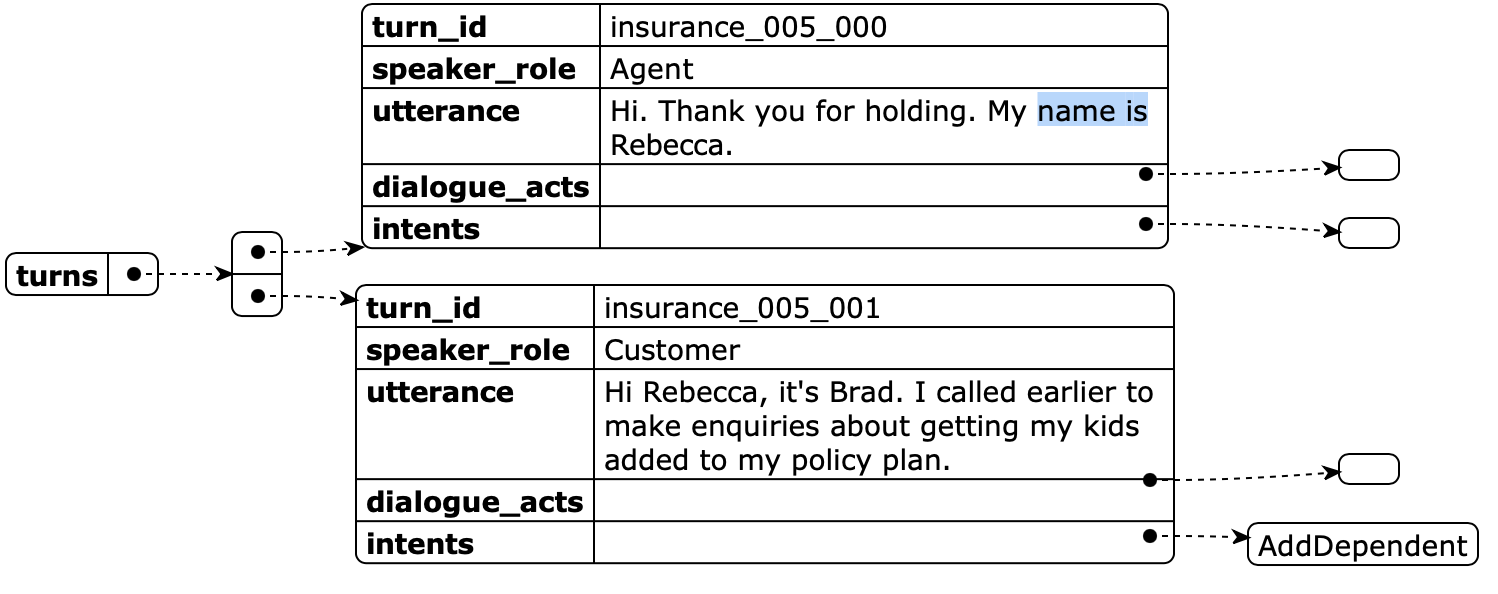
\includegraphics[width=0.75\textwidth]{../images/20221104-234622_screenshot.png}
\end{center}
\end{frame}

\begin{frame}[label={sec:orga808ad0}]{data augmentation using out-domain data}
After getting high quality utterances for sccl(original input in figure), besides drop-out augmentation in sccl, we can augment the original input by simcse using out-domain data(which has similar utterances in original input). Then we can train sccl normally. After getting clustering results, we have to remove the augmentation data added in previous step.
\begin{center}
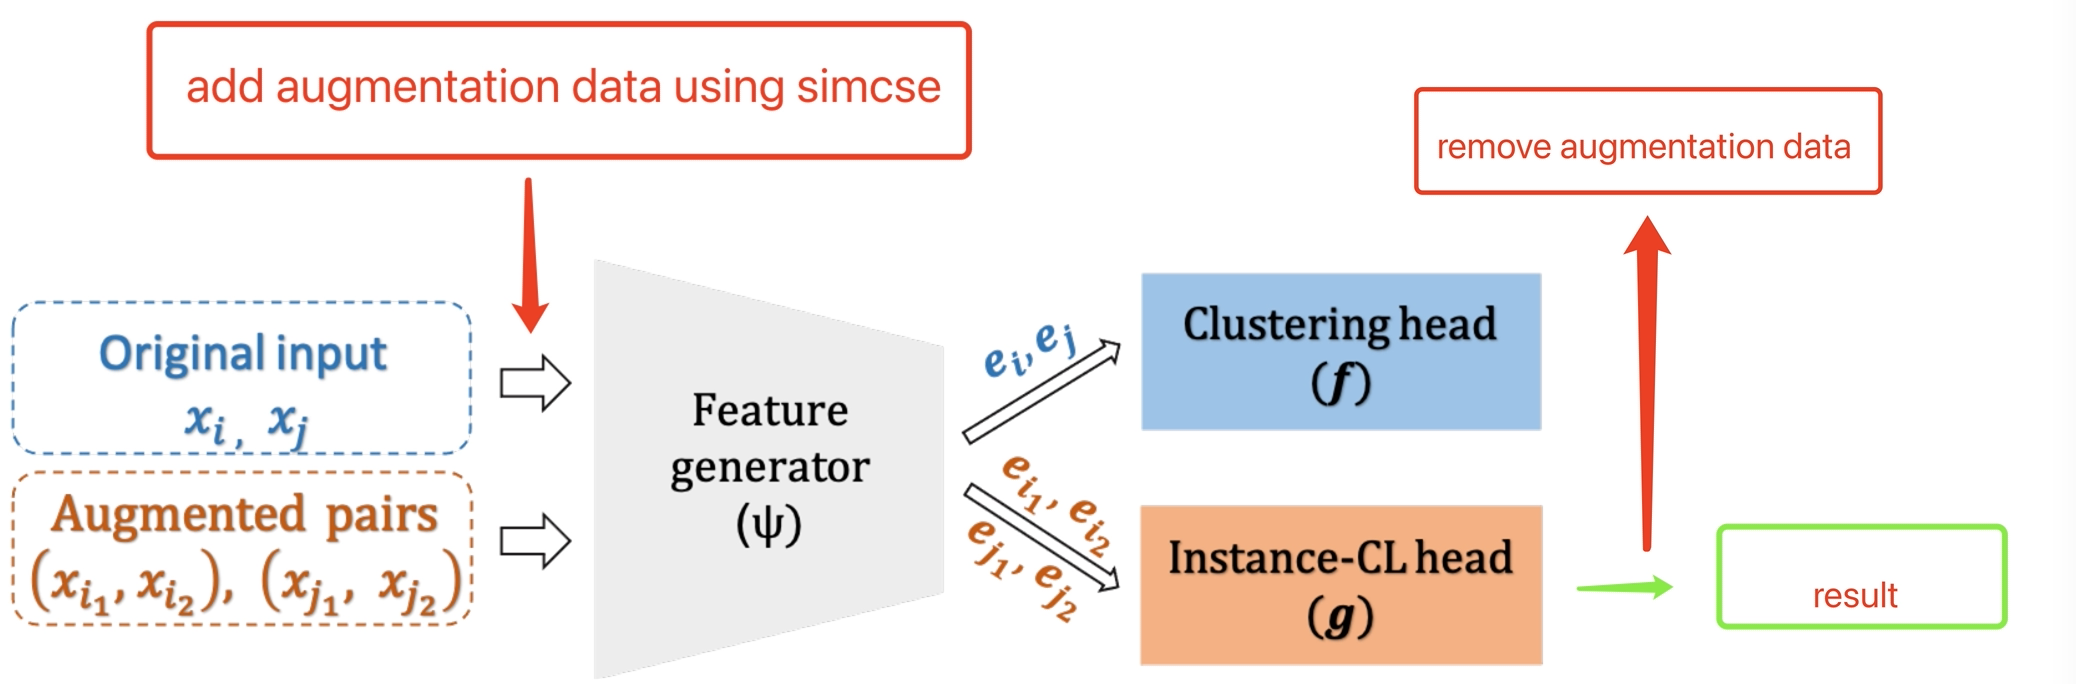
\includegraphics[width=.9\linewidth]{../images/20221104-235604_screenshot.png}
\end{center}
\end{frame}

\begin{frame}[label={sec:org1968ead}]{results}
\begin{center}
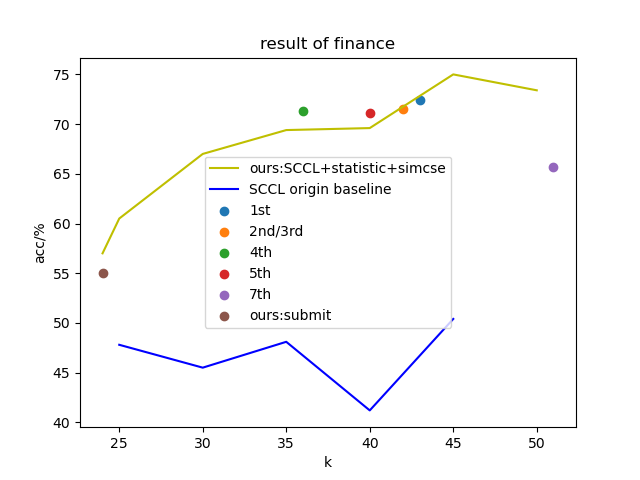
\includegraphics[width=.9\linewidth]{2.png}
\end{center}
\end{frame}
\end{document}